\chapter{\IfLanguageName{dutch}{Stand van zaken}{State of the art}}
\label{ch:stand-van-zaken}

% Tip: Begin elk hoofdstuk met een paragraaf inleiding die beschrijft hoe
% dit hoofdstuk past binnen het geheel van de bachelorproef. Geef in het
% bijzonder aan wat de link is met het vorige en volgende hoofdstuk.

% Pas na deze inleidende paragraaf komt de eerste sectiehoofding.


In dit deel zal er toegespitst worden op de werking van een wayfinding applicatie, bij uitstek de concrete werking van het AI/AR-mechanisme.

\section{Begrippen}
\subsection{AI (Artificiële intelligentie)}
Artificiële intelligentie of AI is een zeer groot fenomeen in de huidige IT-wereld. Het kan worden beschreven als intelligentie die wordt gedemonstreerd door machines. Op deze manier kunnen die apparaten de omgeving waarnemen en vervolgens acties ondernemen die het succesvol bereiken van een bepaald doel zal maximaliseren. In het algemeen staat de term AI ook gekend als de beschrijving van machines of computers die cognitieve acties uitvoeren die wij als mensen associëren met de menselijke geest.

In deze bachelorproef wordt AI toegepast op het vlak van objectdetectie, het is de meest cruciale factor om een wayfinding applicatie te optimaliseren.
Objectdetectie zal in de wayfinding applicatie ervoor zorgen dat de omgeving op een correcte manier wordt herkend, zo kan er een perfect beeld worden geschept van welke objecten de gebruiker afstand moet houden, bijvoorbeeld muren.

\subsubsection{Objectherkenning vs. Objectdetectie}
In Artificiële intelligentie worden twee verschillende manieren gebruikt om objecten te identificeren, objectherkenning en objectdetectie. Het herkenningsproces is zeer gelijkaardig, maar toch zijn er zekere verschillen bij de uitvoering. Objectdetectie kan worden beschouwd als een subset van objectherkenning, de objecten zullen herkend worden op een simultane manier, maar bij objectdetectie wordt het object ook gelokaliseerd in de afbeelding. In de onderstaande afbeelding kan u het verschil duidelijk waarnemen, objectherkenning (links) en objectdetectie (rechts). \autocite{ObjRec2020}

\begin{figure}[H]
	\centering
	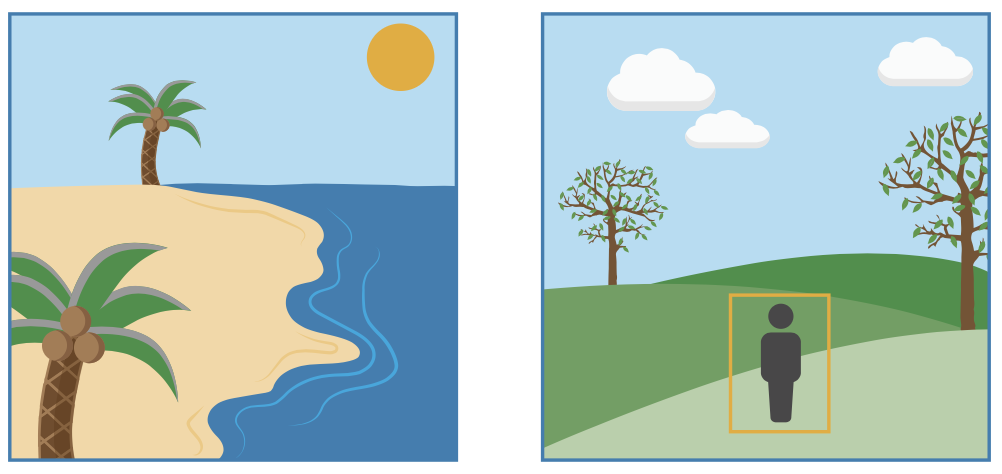
\includegraphics[scale=0.3]{objectdetectie.png}
	\caption{Objectherkenning (links), Objectdetectie (rechts), \autocite{ObjRec2020}}
\end{figure}

\subsection{Werking van objectherkenning}
Om objectherkenning toe te passen kan je gebruik maken van twee verschillende manieren, namelijk 'Machine Learning' en 'Deep learning'. Beide technieken zullen objecten gaan herkennen, maar ze zijn verschillend op vlak van uitvoering.

\subsubsection{Machine learing}
Machine learning maakt gebruik van classificatie om een bepaald object te herkennen. Ten eerste zal de trainingset worden opgesteld, dit gebeurt door een verzameling van afbeeldingen samen te stellen en vervolgens de relevante punten aan te duiden. Het is zeer belangrijk om de juiste relevante punten aan te duiden, anders zal het systeem verkeerd getraind worden, waardoor het algoritme vervolgens een verkeerde output zal geven. Deze punten zullen ervoor zorgen dat het systeem verschillende categorieën herkent. Vervolgens zal het leermodel deze informatie gebruiken om nieuwe objecten (objecten die nog niet gekend zijn in de trainingset) te analyseren en te classificeren. \autocite{ObjRec2020}


\begin{figure}[H]
	\centering
	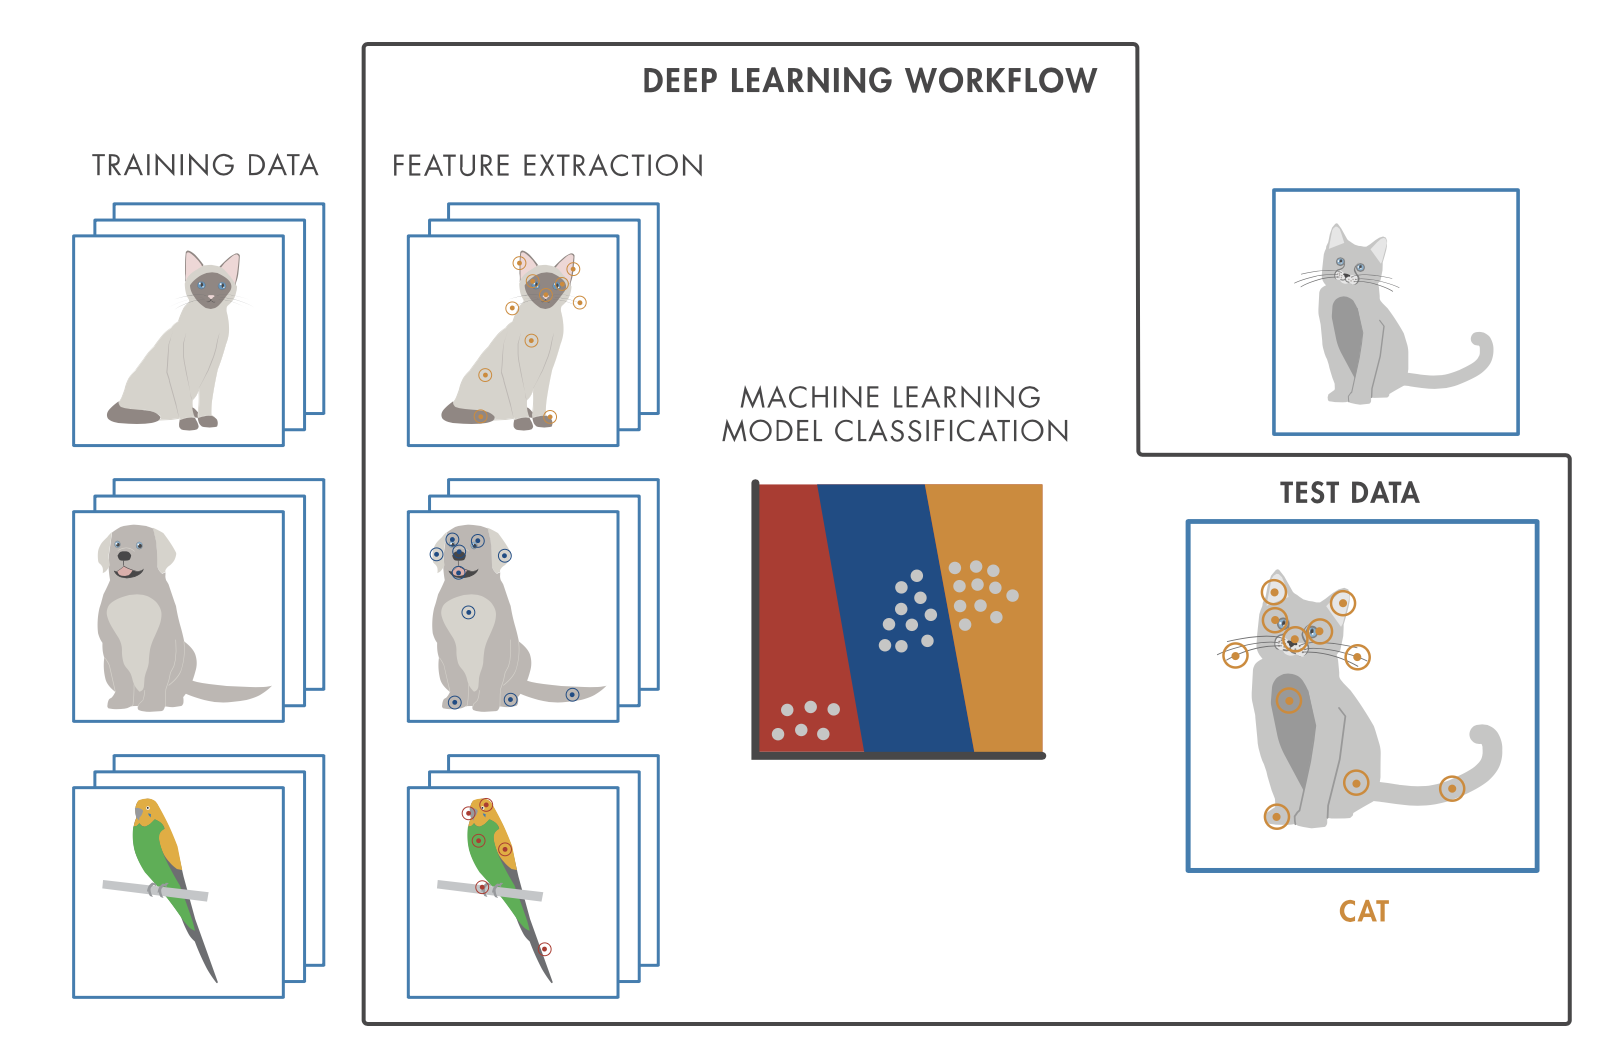
\includegraphics[scale=0.35]{machinelearning.png}
	\caption{Overview Machine learning, \autocite{ObjRec2020}}
\end{figure}


\subsubsection{Deep learning}
Deep learning maakt gebruik van convolutionele neurale netwerken (CNN) om objecten te herkennen. Een CNN kan automatisch de aanhangende kenmerken van een object leren om dat object te identificeren, dit betekent dat een CNN bijvoorbeeld het verschil tussen auto's en vrachtwagens kan herkennen door middel van duizenden afbeeldingen te analyseren en vervolgens te leren welke kenmerken juist verschillend zijn. \autocite{ObjRec2020}

\begin{figure}[H]
	\centering
	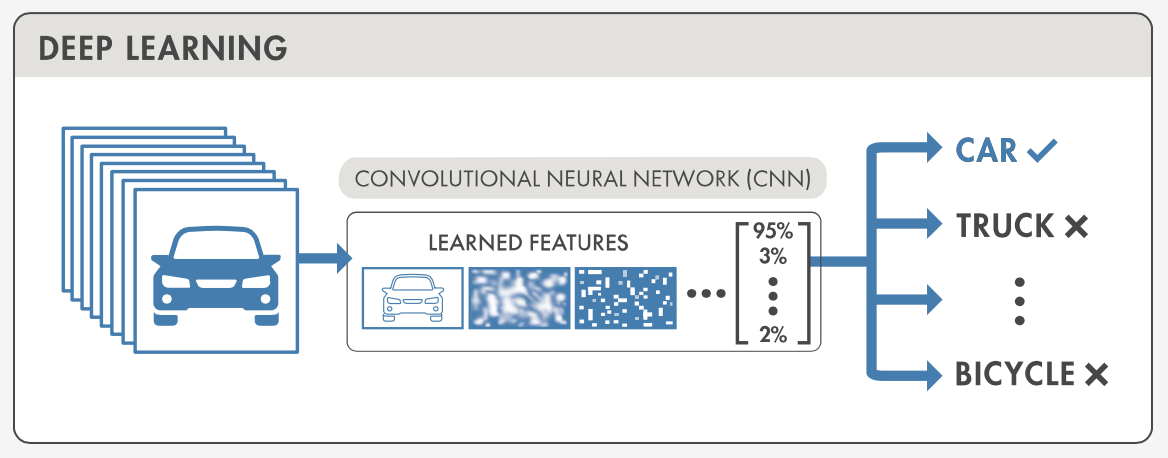
\includegraphics[scale=0.37]{deeplearning.png}
	\caption{Overview Deep learning, \autocite{ObjRec2020}}
\end{figure}

\subsection{AR (Augmented reality)}
Het concept AR is vandaag de dag niet meer uit het straatbeeld weg te denken, het wordt bijvoorbeeld gebruikt bij de Instagram -en Snapchat filters. Augmented reality of AR is een interactieve ervaring met de omgeving waarin objecten die zich in de echte wereld bevinden worden versterkt door computergegenereerde objecten. AR is iets wat al even bestaat, het werd bijvoorbeeld al gebruikt bij één van de eerste straaljagers, het vizier van de piloot wordt in dit voorbeeld ondersteund door een computergegenereerd object dat de vijand zou moeten lokaliseren. Augmented reality werd pas populair bij de modale mens wanneer Naintic Pokemon Go lanceerde, het werd één van de meest gekende smarthonegames. In 2017 introduceerde Android en Apple, AR Core en AR Kit, het werd vervolgens voor developers veel eenvoudiger om AR-applicaties te creëren. \autocite{NewGenApps2017}

Het doel van Augmented reality in deze bachelorproef is om de route op een zo efficiënt mogelijke manier aan te geven, dit betekent dat er geen pijlen door objecten mogen gaan. Om een beeld te kunnen scheppen over het effectieve doeleinde, werd hieronder alvast een voorbeeldfoto toegevoegd.

\begin{figure}[H]
	\centering
	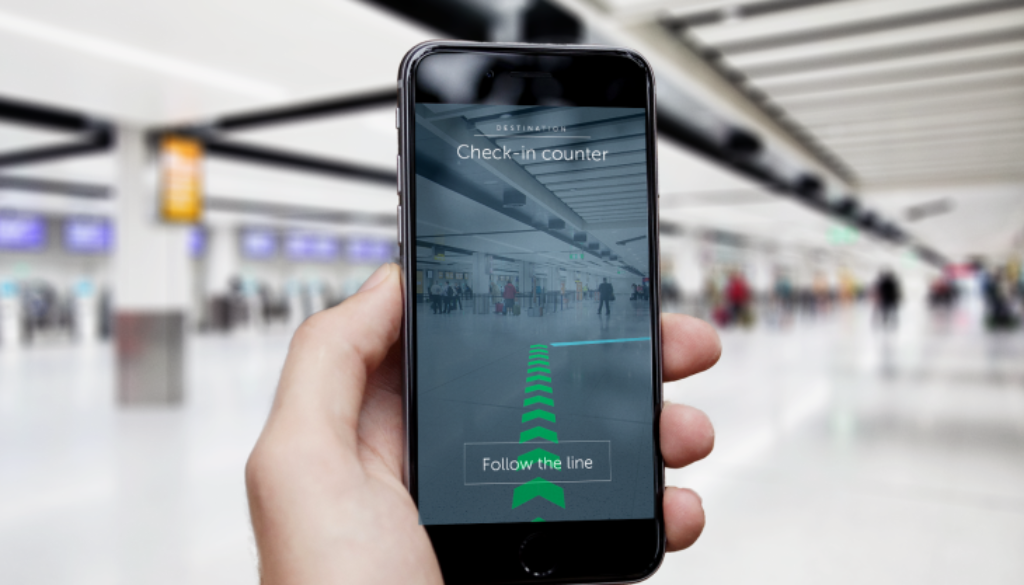
\includegraphics[scale=0.24]{wayfinding.png}
	\caption{Voorbeeld wayfinding applicatie met AR, \autocite{MAXST2019}}
\end{figure}

\subsection{Werking van Augmented reality}
Augmented reality kan momenteel op drie verschillende manieren worden uitgewerkt. Deze verschillende technieken zijn SLAM, herkenning gebaseerd en locatie gebaseerd.

\subsubsection{SLAM (Simultaneous Localization and Mapping)}
Simultaneous Localization and Mapping of SLAM is de manier die het meest effectief en efficiënt werkt. SLAM lokaliseert sensoren ten opzichte van hun omgeving en brengt tegelijkertijd de omgeving in kaart, het is dus een zeer goede aanpak om complexe AR-simulatieproblemen op te lossen. Het SLAM-systeem is in feite een set van algoritmen die gericht zijn op het oplossen van gelijktijdige lokalisatie en het in kaart brengen van problemen. De meeste Augmented realitykits zijn reeds uitgerust met de mogelijkheid tot een SLAM-aanpak. \autocite{NewGenApps2017}

\begin{figure}[H]
	\centering
	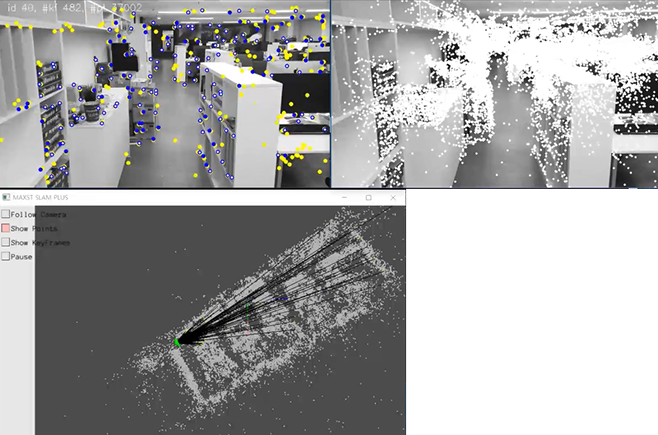
\includegraphics[scale=0.6]{SLAM.png}
	\caption{Voorbeeld SLAM-uitwerking, \autocite{AVRSpot2018}}
\end{figure}

De bovenstaande foto toont een praktische uitwerking van SLAM. In de 2 bovenste foto's ziet u hoe de algoritmen de belangrijkste punten lokaliseren, daaronder ziet u hoe SLAM de omgeving in kaart brengt met behulp van de punten.

\pagebreak
\subsubsection{Herkenning gebaseerd}
Herkenning gebaseerd gebruikt de camera van het gebruikte apparaat om bepaalde visuele markers of objecten te identificeren. Deze AR-technologie is bijgevolg zeer afhankelijk van de kwaliteit van de gebruikte camera, als deze de markers niet goed kan identificeren, dan zal het AR-mechanisme niet goed werken. \autocite{NewGenApps2017}

Bij deze manier is het ook mogelijk om de positie en oriëntatie te berekenen. De markers op het scherm worden vervangen door een overeenkomstig 3D-object, dit maakt het mogelijk om het object meer in detail te bekijken door het bijvoorbeeld te roteren zodat er meerdere invalshoeken kunnen geobserveerd worden.

\subsubsection{Locatie gebaseerd}
Locatie gebaseerd of 'markerless augmented reality' is een AR-technologie die alleen gebruik maakt van een GPS, digitaal kompas, snelheidsmeter of versnellingsmeter om gegevens over de locatie te verzamelen, de augmented reality visualisaties worden met behulp van deze informatie geactiveerd. Een smartphone heeft genoeg sensoren om deze manier te kunnen realiseren. \autocite{NewGenApps2017}

\subsection{AI + AR}
De samenhang van Artificiële intelligentie en Augmented reality is zeer cruciaal bij het optimaliseren van een wayfinding applicatie. Ten eerste is het belangrijk dat de objecten op een correcte manier worden herkend. Ten tweede is het zeer belangrijk dat de bevindingen van de objectherkenning op een correcte manier worden vertaald naar de AR-omgeving. 
\newpage
\section{Verschillende AR en AI frameworks}

\subsection{AR}
Welke AR-kit je juist wilt gebruiken ligt vooral aan u eigen persoonlijke eisen, ze hebben namelijk elk hun specifieke kenmerken. Het bepaalde framework moet ook compatibel zijn met de software die u gebruikt om de applicatie te creëren.
\subsubsection{Unity3D}
Unity3D is zeer populair voor game development, dit framework biedt de oplossing voor elke soort developer, full-stack noch indie \footnote{Indie: individuele of kleine teams van software ontwikkelaars die meestal zonder financiële steun video games creëren.}. Met Unity3D is het ook mogelijk om bepaalde scripts toe te voegen, dit kan worden verstaan als externe voorwerpen zoals stoelen, etc. die  kunnen worden toegevoegd in de virtuele wereld. Unity is zo uitgebreid dat het zelfs mogelijk is om een functionele applicatie te bouwen zonder één regel code te schrijven. Het bedrijf "In The Pocket" (opdrachtgever van bachelorproef) gebruikt inmiddels ook Unity om hun AR-applicaties op te bouwen. Unity is gratis om te gebruiken. \autocite{Arshed2018}

\begin{figure}[H]
	\centering
	
\includegraphics[scale=0.15]{unity.jpg}
	\caption{Logo Unity, \autocite{Unity2019}}
\end{figure}

\subsubsection{Unreal Engine}
Unreal Engine is zoals Unity3D zeer gekend binnen de game development-wereld. Het werd gebruikt bij games zoals Star Trek en Tom Clancy's. Voor Unreal Engine was het vanzelfsprekend dat ze hun framework ook zouden uitbreiden naar 	AR game development. Bij dit framework is het ook mogelijk om externe scripts toe te voegen. Een zeer gegeerd aspect bij software ontwikkelaars is documentatie, dit is in grote mate beschikbaar bij dit framework. Unreal Engine is vervolgens ook gratis, inmiddels wel als de 'Creators License'  wordt gebruikt.  \autocite{Arshed2018}

\begin{figure}[H]
	\centering
	
\includegraphics[scale=0.08]{unrealEngine.jpg}
	\caption{Logo Unreal Engine, \autocite{UnrealEngine2019}}
\end{figure}

\subsubsection{iOS ARKit}
Apple biedt een eigen AR-framework aan zijn developers, namelijk ARKit. Dit framework biedt de mogelijkheid om AR-applicaties te bouwen voor iOS-apparaten. Indien u reeds met Swift heeft gewerkt, dan is dit framework de perfecte oplossing om snel en makkelijk een concrete AR-applicatie te maken. Unity en Unreal Engine maken onderliggend ook gebruik van iOS ARKit om applicaties te deployen naar iOS-toestellen. Net zoals Unity en Unreal Engine is ARKit ook gratis.
\begin{figure}[H]
	\centering
	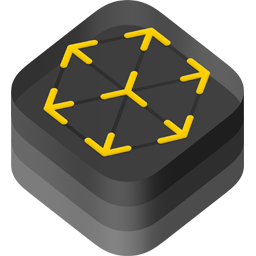
\includegraphics[scale=0.2]{arkit.png}
	\caption{Logo ARKit, \autocite{Apple2019}}
\end{figure}

\subsubsection{Google ARCore}
Google ARCore is een AR-framework dat zowel compatibel is voor Android als iOS. Google lanceerde dit framework na het succesvolle Tango project.
De mogelijkbeid bestaat om andere AR-frameworks zoals Unity, Unreal Engine, etc.  te integreren, door dit aspect wordt ARCore de complete toolkit voor het ontwikkelen van applicaties voor meerdere platformen. Alsook Google ARCore wordt onderliggend gebruikt door Unity en Unreal Engine om applicaties te kunnen deployen naar Android-toestellen. Google ARCore is ook gratis te verkrijgen.

\begin{figure}[H]
	\centering
	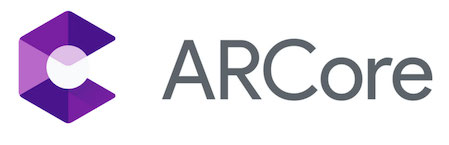
\includegraphics[scale=0.3]{ARCore.jpg}
	\caption{Logo Google ARCore, \autocite{ARCore2019}}
\end{figure}

\subsection{AR + AI}
Het vinden van de perfecte combinatie tussen AR en AI is geen eenvoudige taak en is vaak ook afwisselend van wat het doeleinde is, het artikel van \textcite{Toole2019} (\citetitle{Toole2019}) beschrijft heel duidelijk welke relevante technologiën kunnen worden gebruikt. Er wordt ook besproken hoe geanvanceerd de huidige AI-technieken zijn, deze kunnen namelijk  verticale en horizontale vlakken detecteren, diepte- en segmentbeelden inschatten voor realistische occlusie en zelfs 3D-posities van objecten in real-time afleiden. Deze aspecten zijn zeker van belang voor de wayfinding-applicatie.

De meest gebruikelijke manier om deze 2 technieken (AI en AR) te combineren is door afbeeldingen van een scène te nemen, die gegevens door een AI-model te laten lopen en de modeluitgang te gebruiken om effecten binnen de scène te triggeren. De 2 AI-technieken die worden besproken zijn Core ML en Tensorflow Lite.

De blogpost van \autocite{Girish2020} (\citetitle{Girish2020}) geeft nog een vierde framework waar u zeker rekening mee moet houden, namelijk 'Vuforia'.

\subsubsection{Core ML}
Core ML is een AI-framework dat wordt aangeboden door Apple, dit is vervolgens ook alleen te gebruiken voor iOS-applicaties. Het framework ondersteunt het analyseren van beelden, Natural Language voor het verwerken van tekst, Speech voor het omzetten van audio naar tekst en SoundAnalysis voor het identificeren van geluiden in audio. Core ML zelf bouwt voort op low-level primitieven zoals Accelerate \footnote{Accelerate: framework van Apple dat de mogelijk biedt om grootschalige wiskundige berekeningen en beeldberekeningen uit te voeren met hoge prestaties en een laag energieverbruik.} en BNNS (Basic Neural Network Subroutines) \footnote{BNNS: Basic Neural Network Subroutines is een element binnen Accelerate dat de mogelijkheid biedt om neurale netwerken te gebruiken met eerder verkregen trainingsgegevens.}, evenals Metal Performance Shaders \footnote{Metal Performance Shaders: framework van Apple dat het mogelijk maakt om een goede GPU performantie te crëeren zonder zelfgeschreven 'shaders' te hoeven maken voor elk soort GPU-familie. Een shader is een rendering-algoritme, het zorgt ervoor dat het getoonde beeld op een toestel van goede kwaliteit is.}. Een belangrijke factor is inmiddels ook dat dit framework gratis is. \autocite{AppleML2020}


\begin{figure}[H]
	\centering
	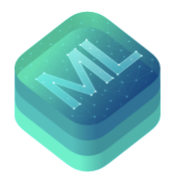
\includegraphics[scale=0.57]{mlcore.png}
	\caption{Logo ML Core, \autocite{AppleML2020}}
\end{figure}

\subsubsection{TensorFlow lite}
TensorFlow is zeer gekend in de AI-wereld, het bedrijf biedt talloze frameworks aan om AI op een eenvoudige manier te integreren in jouw gewenste applicatie. TenserFlow lite werd speciaal gecreëerd om AI te kunnen toepassen met behulp van inputs die worden voorzien door een smartphone, zo is het mogelijk om 'image classification' en 'object detection' toe te passen, met alleen de input van de smartphonecamera. Dit framework is vervolgens ook gratis. \autocite{TensorFlowLite2020}

\begin{figure}[H]
	\centering
	
\includegraphics[scale=0.105]{tensorflowlite.png}
	\caption{Logo TensorFlow Lite, \autocite{TensorFlowLite2020}}
\end{figure}

\subsubsection{Vuforia}
Vuforia is een Augmented Reality SDK (Software development kit) die het voor bedrijven mogelijk maakt om mobiel gerichte, immersieve AR-ervaringen op te bouwen. Vuforia kan gebruikt worden voor iOS -en Androidapplicaties. Deze SDK is niet gratis, het pro-pakket heeft zelfs een relatief hoge prijs voor studenten, maar in dit pakket kan u wel gebruik maken van de reeds geïntegreerde AI-features. \autocite{Girish2020}

\subsubsection{Google Vision API}
Google biedt ook een API (Application programming interface) die het mogelijk maakt om AI te betrekken bij de AR-applicatie. De API werkt als volgt, de applicatie neemt een foto van de waarneming, stuurt deze vervolgens door naar de API en zal daaropvolgend een antwoord bieden waarin de waargenomen objecten worden meegedeeld. Deze API is niet volledig gratis, vanaf een bepaald aantal 'calls' zal er een gepast bedrag moeten worden betaald.

\subsection{Overzicht AR}
\begin{table}[H]
	\centering
	\begin{tabular}{|l|c|c|c|c|}
		\hline
		& \multicolumn{1}{l|}{Unity 3D} & \multicolumn{1}{l|}{Unreal Engine} & \multicolumn{1}{l|}{ARKit} & \multicolumn{1}{l|}{ARCore} \\ \hline
		\textbf{Compatibel met iOS}     & Ja                            & Ja                                 & Ja                         & Ja                          \\ \hline
		\textbf{Compatibel met Android} & Ja                            & Ja                                 & Nee                        & Ja                          \\ \hline
		\textbf{Provider}               & Unity                         & Unreal Engine                      & Apple                      & Google                      \\ \hline
		\textbf{Documentatie}           & Ja                            & Ja                                 & Ja                         & Ja                          \\ \hline
	\end{tabular}
	\caption{Vergelijking AR frameworks}
\end{table}
\pagebreak
\subsection{Overzicht AR + AI}
\begin{table}[H]
	\begin{tabular}{|l|c|c|c|c|}
		\hline
		& Core ML       & TensorFlow lite                                                                    & Vuforia                                                                                                                     & Vision API                                                                            \\ \hline
		\textbf{\begin{tabular}[c]{@{}l@{}}Compatibel met\\  iOS\end{tabular}}             & Ja            & Ja                                                                                 & Ja                                                                                                                          & Ja                                                                                    \\ \hline
		\textbf{\begin{tabular}[c]{@{}l@{}}Compatibel met \\ Android\end{tabular}}         & Nee           & Ja                                                                                 & Ja                                                                                                                          & Ja                                                                                    \\ \hline
		\textbf{Provider}                                                                  & Apple         & TensorFlow                                                                         & Vuforia                                                                                                                     & Google                                                                                \\ \hline
		\textbf{Prijs}                                                                     & Gratis        & Gratis                                                                             & \begin{tabular}[c]{@{}c@{}}Betalend, er \\ zijn 3 pakketten. \\ Basic, \\ Basic + cloud en\\  Pro (incl. AI)\end{tabular} & \begin{tabular}[c]{@{}c@{}}Gratis tot een\\  bepaald aantal \\ API calls\end{tabular} \\ \hline
		\textbf{\begin{tabular}[c]{@{}l@{}}Limiet op (API) \\ calls\end{tabular}}          & Ongelimiteerd & Ongelimiteerd                                                                      & \begin{tabular}[c]{@{}c@{}}Ongelimiteerd, \\ indien u \\ een betalend \\ pakket aanschaft\end{tabular}                    & 1000 / maand                                                                          \\ \hline
		\textbf{\begin{tabular}[c]{@{}l@{}}Compatibel met\\ (AR frameworks):\end{tabular}} & ARKit, Unity3D        & \begin{tabular}[c]{@{}c@{}}Unity3D, Unreal \\ Engine,\\ ARKit, ARCore\end{tabular} & \begin{tabular}[c]{@{}c@{}}Unity3D, maar\\ Vuforia is een\\ AR-SDK op \\ zichzelf\end{tabular}                              & \begin{tabular}[c]{@{}c@{}}Unity3D, Unreal \\ Engine,\\ ARKit, ARCore\end{tabular}    \\ \hline
		\textbf{Documentatie}                                                              & Ja            & Ja                                                                                 & Ja                                                                                                                          & Ja                                                                                    \\ \hline
	\end{tabular}
	\caption{Vergelijking AR + AI frameworks}
\end{table}
\newpage
\section{Bestaand onderzoek}

In deze sectie zal er meer worden gefocust op het onderzoek en de uitwerkingen die reeds werden gerealiseerd. Deze algemene kennis zal gebruikt worden om het onderzoek te ondersteunen. Deze literatuurstudie staat ook in thema van de wayfinding-context, op deze manier is de verkregen informatie relevanter.

In het algemeen kan er besloten worden dat er reeds weinig onderzoek is gedaan naar de samenhang van 'Artificiële intelligentie' en 'Augmented reality' binnen de wayfinding-context. De termen AI en AR zijn afzonderlijk van elkaar zeer gekend in de IT-wereld, men kan dit zelfs niet meer uit het straatbeeld weg denken. Door de grote belangstelling voor AI en AR en de minieme huidige stand-van-zaken binnen de wayfinding-context wordt deze bachelorproef alleen maar interessanter.

\subsection{Artificiële intelligentie (AI)}

\subsubsection{Objectherkenning}
In de uitgave van ~\textcite{Liang2015}, (\citetitle{Liang2015}) werd er onderzoek gedaan naar het gebruik van objectherkenning door middel van 'Convolutionele netwerken' of met andere woorden, 'Deep learning'. De auteurs werden geïnspireerd door 'Deep learning' omdat het reeds meerdere successen had geboekt bij andere computervisietaken. Omdat objectherkenning een zeer belangrijk factor is voor veel complexe systemen, wouden ze dit efficiënter maken en dus ook verbeteren, en dit door gebruik te maken van een geavanceerde techniek, namelijk de convolutionele netwerken. 

Tijdens hun onderzoek werd het netwerk getest door middel van meerdere datasets, namelijk CIFAR-10, CIFAR-100, MNIST en SVHN. Deze datasets zijn zeer handig wanneer er convolutionele netwerken moeten worden getest, u hoeft dus geen data meer te verzamelen om te kunnen observeren of een netwerk wel degelijk goed functioneert. Het vinden van goede datasets is een cruciale factor bij het gebruik van AI, indien deze niet voldoen aan de eisen kunnen er ook geen bruikbare conclusies worden opgesteld.

In het onderzoek wordt er ook nog eens verduidelijkt dat het gebruik van 'Deep learning' zorgt voor betere resultaten. Het verhogen van de parameters in een CNN zorgde in het onderzoek voor een nog betere performantie, in tegenstelling met de 'gewone' feed-forward structuur. 

Uit de conclusie van hun onderzoek kan er besloten worden dat een RCNN (recurrent convolutioneel netwerk) betere resultaten oplevert. Een recurrent convolutioneel netwerk is een uitgebreider CNN, in dit netwerk worden meer recurrente verbindingen (of parameters) toegevoegd in elke laag (zie onderstaande foto). Deze structuur maakte het mogelijk om meer diepgang te creëren, men ging met andere woorden meer informatie verkrijgen uit elke laag, waardoor er meer kans was op het juiste eindresultaat. In de laatste fase van het onderzoek kon er andermaal beslist worden dat het netwerk nog efficiënter werkte door de toevoeging van (nog) meer parameters.

\begin{figure}[H]
	\centering
	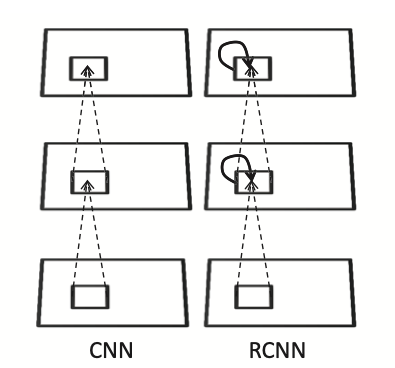
\includegraphics{CNN_RCNN.png}
	\caption{Verschil tussen CNN en RCNN, \autocite{Liang2015}}
\end{figure}

Objectherkenning kan ook rechtstreeks gebruikt worden om de juiste weg te berekenen, dit wordt aangetoond in de studie van \textcite{Haikun2017} (\citetitle{Haikun2017}). In deze paper werd een wayfinding-ontwerp voor een virtuele wereld geoptimaliseerd. Vroeger werd een wayfinding-ontwerp handmatig opgesteld, hierbij moest er rekening worden gehouden met talloze verschillende parameters die mogelijks kunnen veranderen. Zo is het mogelijk dat de menselijke factoren als omgevingsfactoren  kunnen veranderen. Een statisch ontwerp creëren dat steeds voldoet aan relevante eisen is dus niet haalbaar.

Om dit probleem op te lossen werd 'Way to Go!' gecreërd, dit is een systeem dat automatisch een dynamisch wayfinding-ontwerp kan genereren voor verschillende navigatiemogelijkheden. Het systeem werkt als volgt. Ten eerste moet er een navigatiescenario worden gespecificeerd, er zal  met andere woorden een route moeten worden uitgestippeld. Ten tweede zal het systeem automatisch een geoptimaliseerd wayfinding-ontwerp creëren met borden die op de juiste manier zijn geplaatst, rekening houdend met de zichtbaarheid van menselijke agenten en de mogelijkheid om fouten te maken tijdens een navigatie.  In het onderzoek worden de resultaten geëvalueerd door verschillende wayfinding-ontwerpen te vergelijken. Het onderzoek laat vervolgens ook zien dat het geoptimaliseerde wayfinding-ontwerp voetgangers effectief en efficiënt naar hun bestemming kan leiden. De aanpak kan de ontwerper ook helpen om de bereikbaarheid van een bestemming vanaf verschillende locaties te visualiseren en eventuele 'blinde' zones te corrigeren met extra bewegwijzering.

In de onderstaande foto wordt het experiment verder verduidelijkt, de verschillende foto's vertonen de resultaten tijdens elke stap van het onderzoek.

\begin{figure}[H]
	\centering
	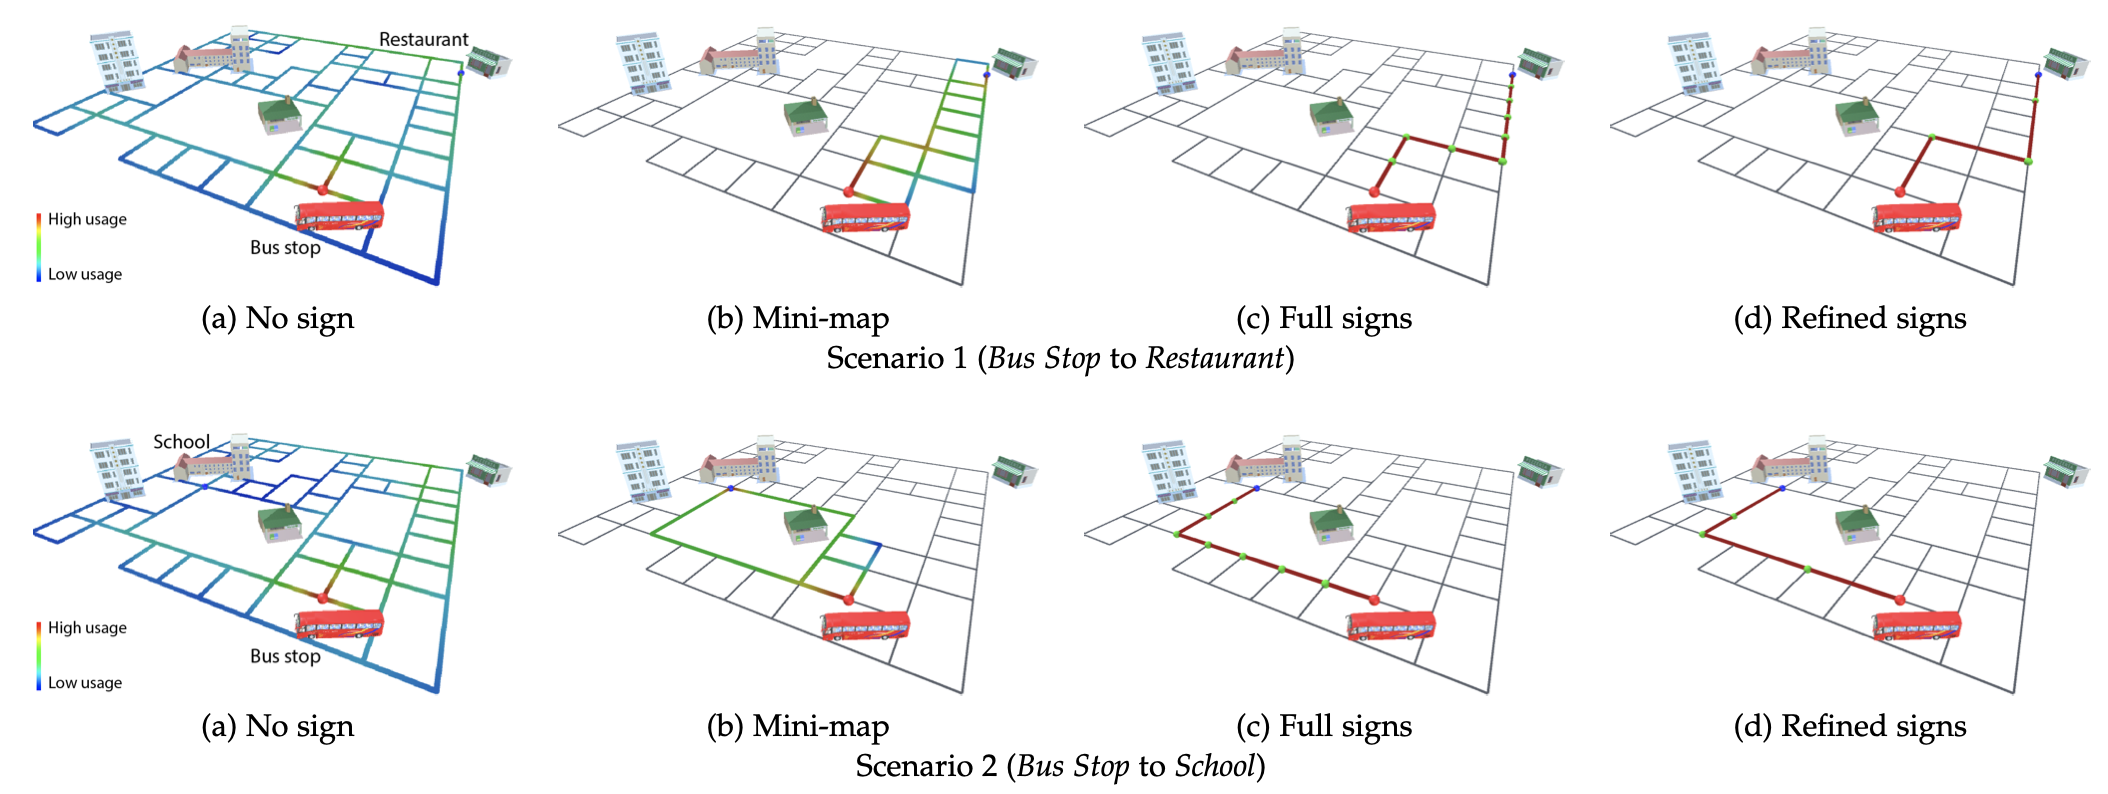
\includegraphics[scale=0.4]{WayToGo.png}
	\caption{Way To Go , \autocite{Haikun2017}}
\end{figure}

\subsubsection{Postionering}
Positionering binnenin gebouwen is zeer belangrijk in de wayfinding-context, als er niet goed kan bepaald worden waar de gebruiker zich bevindt, dan is het zeker niet mogelijk om de gepaste route aan te tonen. Het onderzoek van \textcite{Hasan2019} (\citetitle{Hasan2019}) biedt hier een mogelijke oplossing voor. Zij hebben verschillende 'draadloze' technieken onderzocht die de locatie binnenshuis kunnen bepalen. De traditionele GPS (Global positioning system) is wel gekend om de locatie buitenshuis te bepalen, maar deze voldoet meestal niet aan de benodigdheden voor binnenhuispositionering. De huidige technologie die hiervoor gekend staat is Wi-Fi positionering.

In deze paper beschrijven de auteurs hoe de 'indoor' positie kan bepaald worden door middel van Wi-Fi, Bluetooth en Radio-frequency Idenfication Service (RFID). Deze hebben ze ook uitgewerkt voor verschillende doelapplicaties die steeds gekoppeld zijn aan een bepaalde sector, bv. marketing and customer assistance, health sector, security, ...

Uit hun conclusie kan er worden besloten dat de nauwkeurigheid van de plaatsbepaling deels afhangt van de dichtheid van de toegangspunten en de standaardisatiepunten. Deze informatie kan van pas komen in typische openbare gebouwen zoals winkelcentra, universiteiten en luchthavens. In hun onderzoek werden ze ook geconfronteerd met bepaalde uitdagingen. Zo constateerden zij dat de resolutie van de plaatsbepaling drastisch verslechtert wanneer het gebruik maakt van een non-LOS multipath. Non-line-of-sight of (non-LOS) zijn radiotransmissies (signalen) die worden geblokkeerd door een fysiek object, in het geval van dit onderzoek zouden dat bijvoorbeeld muren kunnen zijn. Om dit soort problemen op te lossen worden 'multipath'-propagatiemethodes gebruikt, in dit geval worden de radiosignalen van andere nabijgelegen objecten afgestoten om toch bij de ontvanger te komen. In de onderstaande foto kan u de 'multipath'-propogatiemethode waarnemen, in deze GPS-context zijn de blauwe lijnen deel van het 'multipath'. In het onderzoek werden vervolgens enkele oplossingen voorgesteld die kunnen helpen bij de aanpak van deze uitdaging.

\begin{figure}[H]
	\centering
	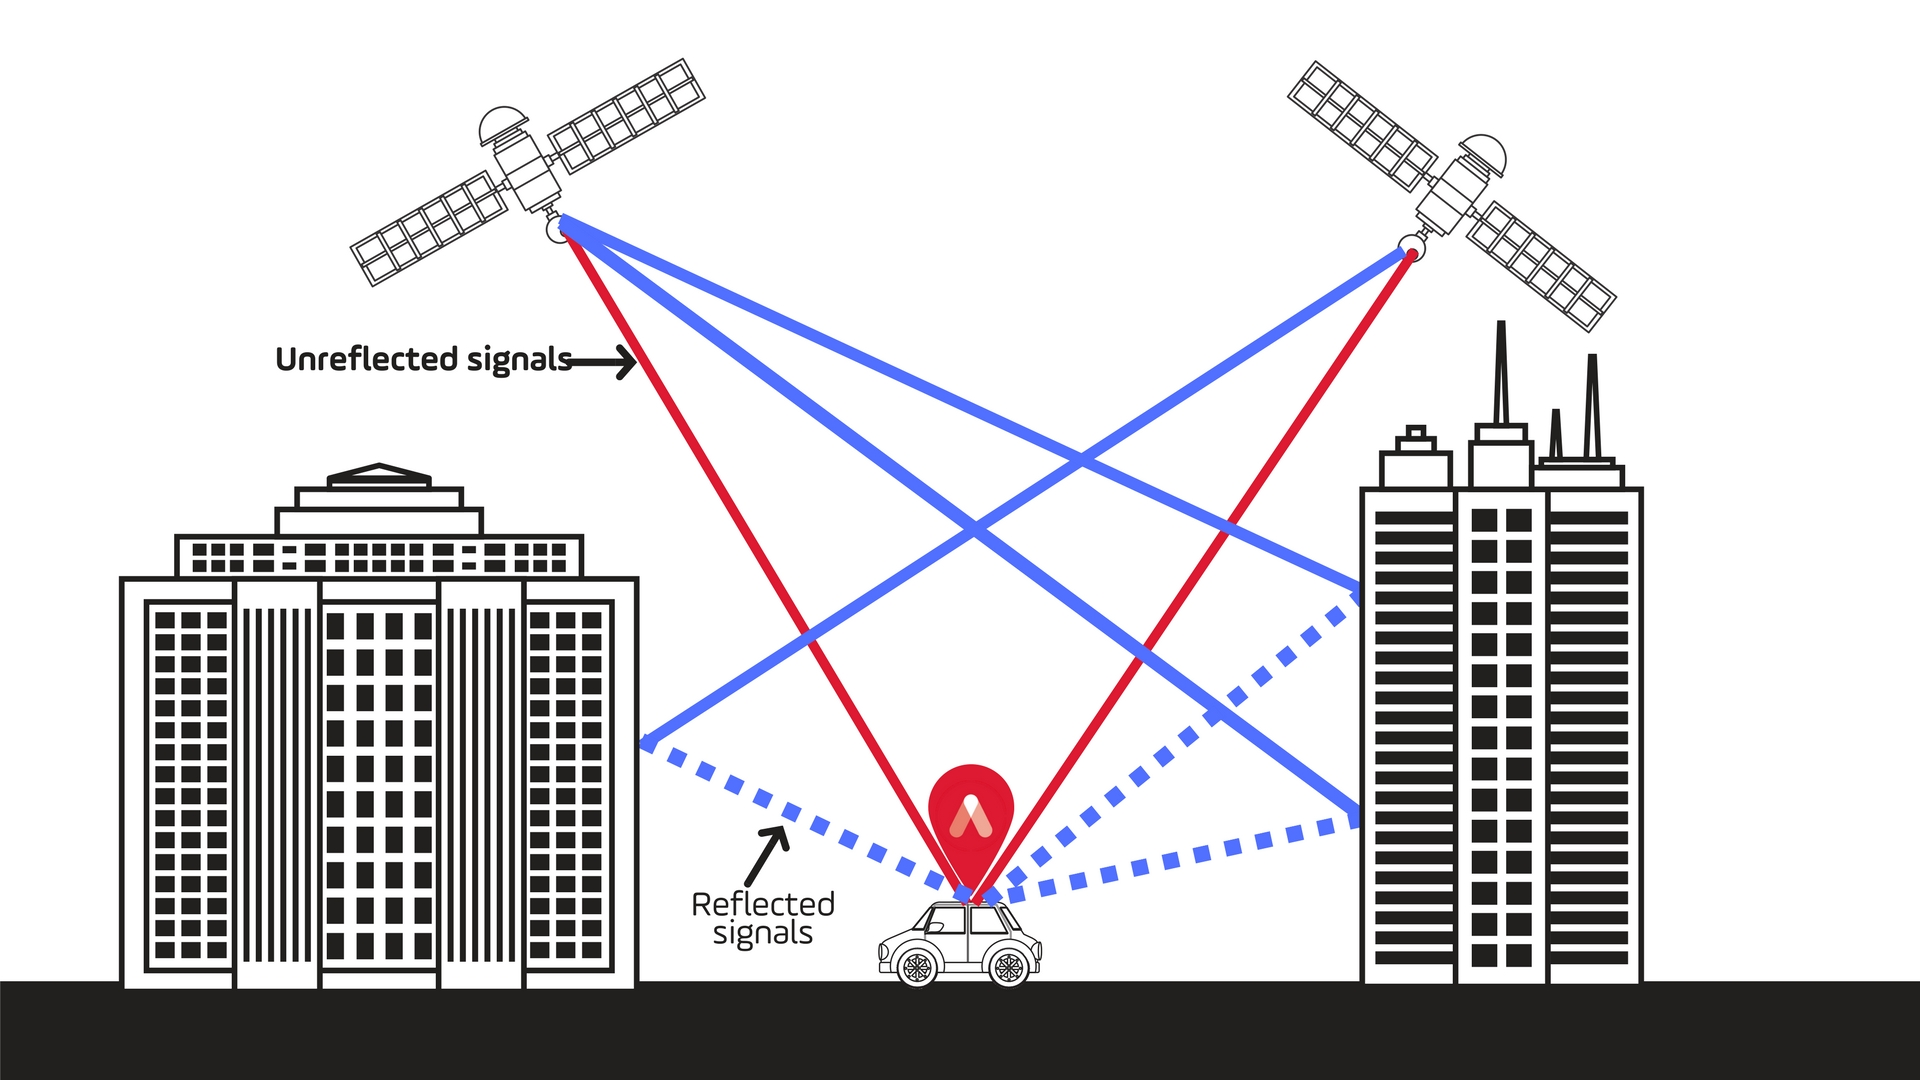
\includegraphics[scale=0.2]{MultiPathPropogation.jpg}
	\caption{GPS multipath, \autocite{Haikun2017}}
\end{figure}


\subsection{Augmented reality (AR)}

\subsubsection{Simultaneous Localization and Mapping (SLAM)}
Het onderzoek van \textcite{Zhang2017} (\citetitle{Zhang2017}) heeft als hoofddoel om het leven voor slechtzienden makkelijker te maken. Ze wensten dit doel te bereiken door een indoor wayfinding applicatie te creëren die deze bepaalde groep mensen zal begeleiden bij het vinden van de weg, specifiek in gebouwen. Dit onderzoek is zeer vergelijkbaar met deze bachelorproef, het eindproduct kent namelijk een grote gelijkenis, alleen wordt er in deze paper gebruik gemaakt van audio-ondersteuning. De resultaten uit deze publicatie zullen met zekerheid helpen bij het vinden van het gepaste eindresultaat.

In dit onderzoek probeerden de auteurs de huidige SLAM-technieken te verbeteren, volgens de state-of-the-art werden er steeds fouten gevonden bij het bepalen van de correcte positie, de zogekende 6-DOF-fout \footnote{6-DOF: 6 Degrees Of Freedom verwijst naar de bewegingsvrijheid van een object binnen een driedimensionale ruimte.}. De gekende aanpassingen die werden toegepast tijdens het onderzoek verbeterden niet alleen de 6-DOF-fout, maar ook de rekentijd. Dit resulteert in een snellere response naar de eindgebruiker, wat alleen maar een positieve invloed heeft op de gebruiksvriendelijkheid. In het onderzoek werden ook experimenten uitgevoerd, deze toonden daadwerkelijk aan dat de effectiviteit van het navigeren wel degelijk werd verbeterd voor slechtziende mensen.

\subsection{Artificiële intelligentie (AI) + Augmented reality (AR)}
\subsubsection{Uitgewerkte wayfinding applicatie}
De paper van \textcite{Pouria2016} (\citetitle{Pouria2016}) zal zeer veel hulp bieden, het eindresultaat van dit onderzoek kent namelijk een zeer grote overeenkomst met de objectieven van deze bachelorproef. Dit onderzoek gebruikt evenals hetzelfde soort toestel om te communiceren met de gebruiker.

In de uitwerking hielden ze rekening met de sensoren die zich bevinden in mobiele toestellen, hiermee gingen ze ook aan de slag. Deze sensoren hebben het mogelijk gemaakt om de locatie, koers en oriëntatie van de gebruiker te detecteren en om contextuele informatie uit verschillende bronnen van online gegevens te verkrijgen. Het combineren van de verkregen data van positionerings- en oriëntatiesensoren met camera's heeft het ook mogelijk gemaakt om praktische Augmented Reality (AR)-toepassingen op deze mobiele apparaten in te zetten. 

Voor de uitwerking van de paper werd een systeem gecreëerd dat een beeld geeft over de navigatiebeleving, dit werd gerealiseerd door middel van Augmented reality en continue feedback van de gebruiker ten opzichte van de dichtstbijzijnde oriëntatiepunten. Deze oriëntatiepunten zijn nodig voor de navigatie en om het juiste pad te vinden. De exacte positie werd bepaald door middel van GPS-sensoren, deze zijn reeds aanwezig in mobiele apparaten. Bovenop de GPS-data werd ook gebruik gemaakt van een beeldverwerkingsalgoritme die de juiste afstand berekent tot een oriëntatiepunt. Om de effectiviteit van het padvinden te verbeteren werd een machinaal leeralgoritme toegevoegd. Dit algoritme zal ervoor zorgen dat het voor elke gebruiker een bewegingsprofiel kan opstellen, dit profiel zal ervoor zorgen dat het steeds aanpassingen kan uitvoeren op de navigatie-instructies.

Uit de experimenten werd gebleken dat het gebruikte algoritme veel betere resultaten leverde als een 'normaal' turn-by-turn systeem, deze technologie wordt gebruikt bij de huidige GPS-toestellen.

\subsubsection{Dent Reality}
Dent Reality is een start-up die gevestigd is in Londen, ze specialiseren zich in het maken van indoor AR-navigatiesystemen voor winkelcentrums en andere grote ruimtes. Het product dat ze leveren is identiek met het doeleinde van deze bachelorproef. De wayfinding-applicatie maakt ook gebruik van machine learning om de locatie en navigatie te optimaliseren.

In het artikel van \textcite{Hart2019} (\citetitle{Hart2019}) wordt besproken hoe ze de applicatie tot stand hebben gebracht, inclusief motivatie. Er kan besloten worden dat vele challenges die worden besproken in het artikel terugkomen in de voorgaande elementen van deze literatuurstudie. De uitwerking van Dent Reality zal met garantie een belangrijke bron van informatie zijn in het komende onderzoek.

\begin{figure}[H]
	\centering
	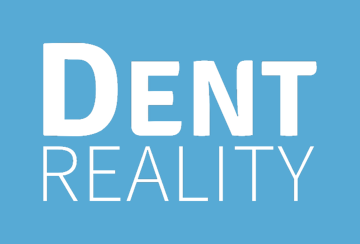
\includegraphics[scale=0.5]{dentReality.png}
	\caption{Logo Dent Reality, \autocite{Hart2019}}
\end{figure}

